\documentclass{jarticle}
\usepackage{graphicx}
\begin{document}
\section{ナビエ・ストークス方程式系の離散化}
非圧縮性の粘性流体の挙動を数理的にとらえるためには、ナビエ・ストークス方程
式と非圧縮性より導かれる連続の方程式とを連立した上で、 初期条件や境界条件を
与えて解くことになる。 ナビエ・ストークス方程式に非圧縮性の条件式を連立させた
方程式をナビエ・ストークス方程式系と呼ぶ。


\begin{equation}
\left.
\begin{tabular}{l}
$\displaystyle
\frac{\partial u}{\partial t}+u\frac{\partial u}{\partial x}+v\frac{\partial u}{\partial y} = -\frac{\partial p}{\partial x}+\frac{1}{Re}(\frac{\partial^2 u}{\partial x^2}+\frac{\partial^2 u}{\partial y^2})+X$\\
$\displaystyle  
\frac{\partial v}{\partial t}+u\frac{\partial v}{\partial x}+v\frac{\partial v}{\partial y} = -\frac{\partial p}{\partial y}+\frac{1}{Re}(\frac{\partial^2 v}{\partial x^2}+\frac{\partial^2 v}{\partial y^2})+Y$
\end{tabular}
\right\}
\end{equation}

\theequation はナビエ・ストークス方程式(勾配型),

\begin{equation}
\displaystyle
  \frac{\partial u}{\partial x}+\frac{\partial v}{\partial y} = 0
\end{equation}

\theequation は連続の方程式である。

上記の速度(U)と圧力(P)を未知量とする定式化を原始変数法(primitive variable method)と呼ぶ。2次元から3次元への拡張も可能である。

これに対して、渦度と流れ関数を用いる表現に流れ関数渦度法がある。
離散化した時の行列次元が小さい、及び連続の方程式を厳密に満たすというメリット
があるが、2次元解析にしか用いることが出来ない。


\section{弱形式の導出}

有限要素法による離散化の基礎となる弱形式を導く。
ナビエ・ストークス方程式の第1式、第2式に対する重み関数をそれぞれ
$u^*$、$v^*$とし、連速の方程式に対する重み関数を$p^*$とする。

ここに$u$は、$x$軸方向の速度成分、$v$は$y$軸方向の速度成分であるから、
重み関数$u^*$、$v^*$も同じ関数形であると仮定する。

また、連続の方程式は圧力$p$のため式と考える。

ナビエ・ストークス方程式の1、2式にそれぞれ$u^*$、$v^*$を乗じ、
連続の方程式に$p^*$を乗じると次の3式になる。


\begin{equation}
\left.
\begin{tabular}{l}
$\displaystyle
u^*\left[\frac{\partial u}{\partial t}+u\frac{\partial u}{\partial x}+v\frac{\partial u}{\partial y}+\frac{\partial p}{\partial x}-\frac{1}{Re}(\frac{\partial^2 u}{\partial x^2}+\frac{\partial^2 u}{\partial y^2})-X\right]=0$\\
$\displaystyle  
v^*\left[\frac{\partial v}{\partial t}+u\frac{\partial v}{\partial x}+v\frac{\partial v}{\partial y}+\frac{\partial p}{\partial y}-\frac{1}{Re}(\frac{\partial^2 v}{\partial x^2}+\frac{\partial^2 v}{\partial y^2})-Y\right]=0$
\end{tabular}
\right\}
\end{equation}

\theequation はナビエ・ストークス方程式(勾配型),

\begin{equation}
\displaystyle
p^*\left(\frac{\partial u}{\partial x}+\frac{\partial v}{\partial y}\right) = 0
\end{equation}

\theequation は連続の方程式である。


上の3本の式を計算領域$\Omega$で積分する。



\begin{equation}
\left.
\begin{tabular}{l}
$\displaystyle
\int\int_\Omega u^*\left[\frac{\partial u}{\partial t}+u\frac{\partial u}{\partial x}+v\frac{\partial u}{\partial y}+\frac{\partial p}{\partial x}-\frac{1}{Re}(\frac{\partial^2 u}{\partial x^2}+\frac{\partial^2 u}{\partial y^2})-X\right]dxdy=0$\\
$\displaystyle  
\int\int_\Omega v^*\left[\frac{\partial v}{\partial t}+u\frac{\partial v}{\partial x}+v\frac{\partial v}{\partial y}+\frac{\partial p}{\partial y}-\frac{1}{Re}(\frac{\partial^2 v}{\partial x^2}+\frac{\partial^2 v}{\partial y^2})-Y\right]dxdy=0$
\end{tabular}
\right\}
\end{equation}

\theequation はナビエ・ストークス方程式(勾配型),

\begin{equation}
\displaystyle
\int\int_\Omega p^*\left(\frac{\partial u}{\partial x}+\frac{\partial v}{\partial y}\right)dxdy = 0
\end{equation}

\theequation は連続の方程式である。

ガウスの発散定理を用いて、
(5)(6)左辺の圧力項と粘性応力項(Reを含む項)を部分積分し、
以下の境界条件(9)を考慮する。

\begin{equation}
\begin{tabular}{ll}
  $\displaystyle
  u = \hat u, v = \hat v $&$on~~~ (\Gamma_1 上 流入境界条件)$\\
\end{tabular}
\end{equation}
\begin{equation}
\begin{tabular}{ll}
  $\displaystyle
  u = v = 0 $&$on~~~ (\Gamma_2 上 ディレクレ境界条件)$\\
\end{tabular}
\end{equation}
\begin{equation}
\begin{tabular}{ll}
$\displaystyle
  -pn_x+\frac{1}{Re}\frac{\partial u}{\partial n} = -pn_y+\frac{1}{Re}\frac{\partial v}{\partial n}=0 $&$on~~~ (\Gamma_3 上 ノイマン境界条件)$
\end{tabular}
\end{equation}


\begin{equation}
\begin{tabular}{l}
$\displaystyle
\int\int_\Omega u^*\left(\frac{\partial u}{\partial t}+u\frac{\partial u}{\partial x}+v\frac{\partial u}{\partial y}\right)dxdy - \int\int_\Omega\frac{\partial u^*}{\partial x}pdxdy
$
\\
$\displaystyle
+\frac{1}{Re}\int\int_\Omega\left(\frac{\partial u^*}{\partial x}\frac{\partial u}{\partial x}+\frac{\partial u^*}{\partial y}\frac{\partial u}{\partial y}\right)dxdy-\int\int_\Omega u^*Xdxdy
$
\\
$\displaystyle
-\int_{\Gamma_1+\Gamma_2}u^*\left(\-pn_x+\frac{1}{Re}\frac{\partial u}{\partial n}\right)d\Gamma = 0
$
\end{tabular}
\end{equation}

\begin{equation}
\begin{tabular}{l}
$\displaystyle
\int\int_\Omega v^*\left(\frac{\partial v}{\partial t}+u\frac{\partial v}{\partial x}+v\frac{\partial v}{\partial y}\right)dxdy - \int\int_\Omega\frac{\partial v^*}{\partial x}pdxdy
$
\\
$\displaystyle
+\frac{1}{Re}\int\int_\Omega\left(\frac{\partial v^*}{\partial x}\frac{\partial v}{\partial x}+\frac{\partial v^*}{\partial y}\frac{\partial v}{\partial y}\right)dxdy-\int\int_\Omega v^*Ydxdy
$
\\
$\displaystyle
-\int_{\Gamma_1+\Gamma_2}v^*\left(\-pn_y+\frac{1}{Re}\frac{\partial v}{\partial n}\right)d\Gamma = 0
$
\end{tabular}
\end{equation}

この時点で、(10)(11)を満たす$uvp$を弱解(weak solution)と呼ぶ、
$uvp$に十分な滑らさがなくて、
(1)(2)を満たすことはなくても、(10)(11)を満足する解も考えることが
できるからである。
これに対して、(1)(2)を満たす解$uvp$は(10)(11)をも満たすが、これは
強解(strong solution)と呼ぶ。


(10)(11)に境界条件(7)(8)を考慮すると、$\Gamma_1$と$\Gamma_2$上では
$u^*=v^*=0$とおくことができるので、(10)(11)の線積分の項は消えてくれる。
そして次式のようになる。



\begin{equation}
\begin{tabular}{l}
$\displaystyle
\int\int_\Omega u^*\left(\frac{\partial u}{\partial t}+u\frac{\partial u}{\partial x}+v\frac{\partial u}{\partial y}\right)dxdy - \int\int_\Omega\frac{\partial u^*}{\partial x}pdxdy
$
\\
$\displaystyle
+\frac{1}{Re}\int\int_\Omega\left(\frac{\partial u^*}{\partial x}\frac{\partial u}{\partial x}+\frac{\partial u^*}{\partial y}\frac{\partial u}{\partial y}\right)dxdy-\int\int_\Omega u^*Xdxdy=0
$
\end{tabular}
\end{equation}

\begin{equation}
\begin{tabular}{l}
$\displaystyle
\int\int_\Omega v^*\left(\frac{\partial v}{\partial t}+u\frac{\partial v}{\partial x}+v\frac{\partial v}{\partial y}\right)dxdy - \int\int_\Omega\frac{\partial v^*}{\partial x}pdxdy
$
\\
$\displaystyle
+\frac{1}{Re}\int\int_\Omega\left(\frac{\partial v^*}{\partial x}\frac{\partial v}{\partial x}+\frac{\partial v^*}{\partial y}\frac{\partial v}{\partial y}\right)dxdy-\int\int_\Omega v^*Ydxdy=0
$
\end{tabular}
\end{equation}

数式(12)(13)(6)が数式(1)(2)の弱形式である。

\section{弱形式の離散化}


$\Omega_e$をe番目の三角形要素の内部領域を表すとすると、
$1\leq e \leq N(総要素数)$なるeに対して、
以下の数式(14)(15)(16)が成り立つ。


\begin{equation}
\begin{tabular}{l}
$\displaystyle
\int\int_{\Omega_e} u^*\left(\frac{\partial u}{\partial t}+u\frac{\partial u}{\partial x}+v\frac{\partial u}{\partial y}\right)dxdy - \int\int_{\Omega_e}\frac{\partial u^*}{\partial x}pdxdy
$
\\
$\displaystyle
+\frac{1}{Re}\int\int_{\Omega_e}\left(\frac{\partial u^*}{\partial x}\frac{\partial u}{\partial x}+\frac{\partial u^*}{\partial y}\frac{\partial u}{\partial y}\right)dxdy-\int\int_{\Omega_e} u^*Xdxdy=0
$
\end{tabular}
\end{equation}

\begin{equation}
\begin{tabular}{l}
$\displaystyle
\int\int_{\Omega_e} v^*\left(\frac{\partial v}{\partial t}+u\frac{\partial v}{\partial x}+v\frac{\partial v}{\partial y}\right)dxdy - \int\int_{\Omega_e}\frac{\partial v^*}{\partial x}pdxdy
$
\\
$\displaystyle
+\frac{1}{Re}\int\int_{\Omega_e}\left(\frac{\partial v^*}{\partial x}\frac{\partial v}{\partial x}+\frac{\partial v^*}{\partial y}\frac{\partial v}{\partial y}\right)dxdy-\int\int_{\Omega_e} v^*Ydxdy=0
$
\end{tabular}
\end{equation}


\begin{equation}
\displaystyle
\int\int_{\Omega_e} p^*\left(\frac{\partial u}{\partial x}+\frac{\partial v}{\partial y}\right)dxdy = 0
\end{equation}


各三角形要素$\Omega_e$において数式(14)(15)(16)が成り立っているのだから、
全ての三角形要素$\Omega_1,\Omega_2,...\Omega_N$において総和を取った
以下の式が成り立つ。


\begin{equation}
\begin{tabular}{l}
$\displaystyle
\sum_{e=1}^N\left[\int\int_{\Omega_e} u^*\left(\frac{\partial u}{\partial t}+u\frac{\partial u}{\partial x}+v\frac{\partial u}{\partial y}\right)dxdy - \int\int_{\Omega_e}\frac{\partial u^*}{\partial x}pdxdy\right.
$
\\
$\displaystyle
\left.+\frac{1}{Re}\int\int_{\Omega_e}\left(\frac{\partial u^*}{\partial x}\frac{\partial u}{\partial x}+\frac{\partial u^*}{\partial y}\frac{\partial u}{\partial y}\right)dxdy-\int\int_{\Omega_e} u^*Xdxdy\right]=0
$
\end{tabular}
\end{equation}

\begin{equation}
\begin{tabular}{l}
$\displaystyle
\sum_{e=1}^N\left[\int\int_{\Omega_e} v^*\left(\frac{\partial v}{\partial t}+u\frac{\partial v}{\partial x}+v\frac{\partial v}{\partial y}\right)dxdy - \int\int_{\Omega_e}\frac{\partial v^*}{\partial x}pdxdy\right.
$
\\
$\displaystyle
\left.+\frac{1}{Re}\int\int_{\Omega_e}\left(\frac{\partial v^*}{\partial x}\frac{\partial v}{\partial x}+\frac{\partial v^*}{\partial y}\frac{\partial v}{\partial y}\right)dxdy-\int\int_{\Omega_e} v^*Ydxdy\right]=0
$
\end{tabular}
\end{equation}


\begin{equation}
\displaystyle
\sum_{e=1}^N\left[\int\int_{\Omega_e} p^*\left(\frac{\partial u}{\partial x}+\frac{\partial v}{\partial y}\right)dxdy\right] = 0
\end{equation}

領域$\Omega_e$における流速と圧力の離散化を行うため、面積座標を導入する。
それから、C++との関係を確認した上で、面積座標を用いた形状関数ベクトルを用いて離散化の続きを行う。

\section{面積座標の定義}

\begin{figure}[h]
\begin{center} 
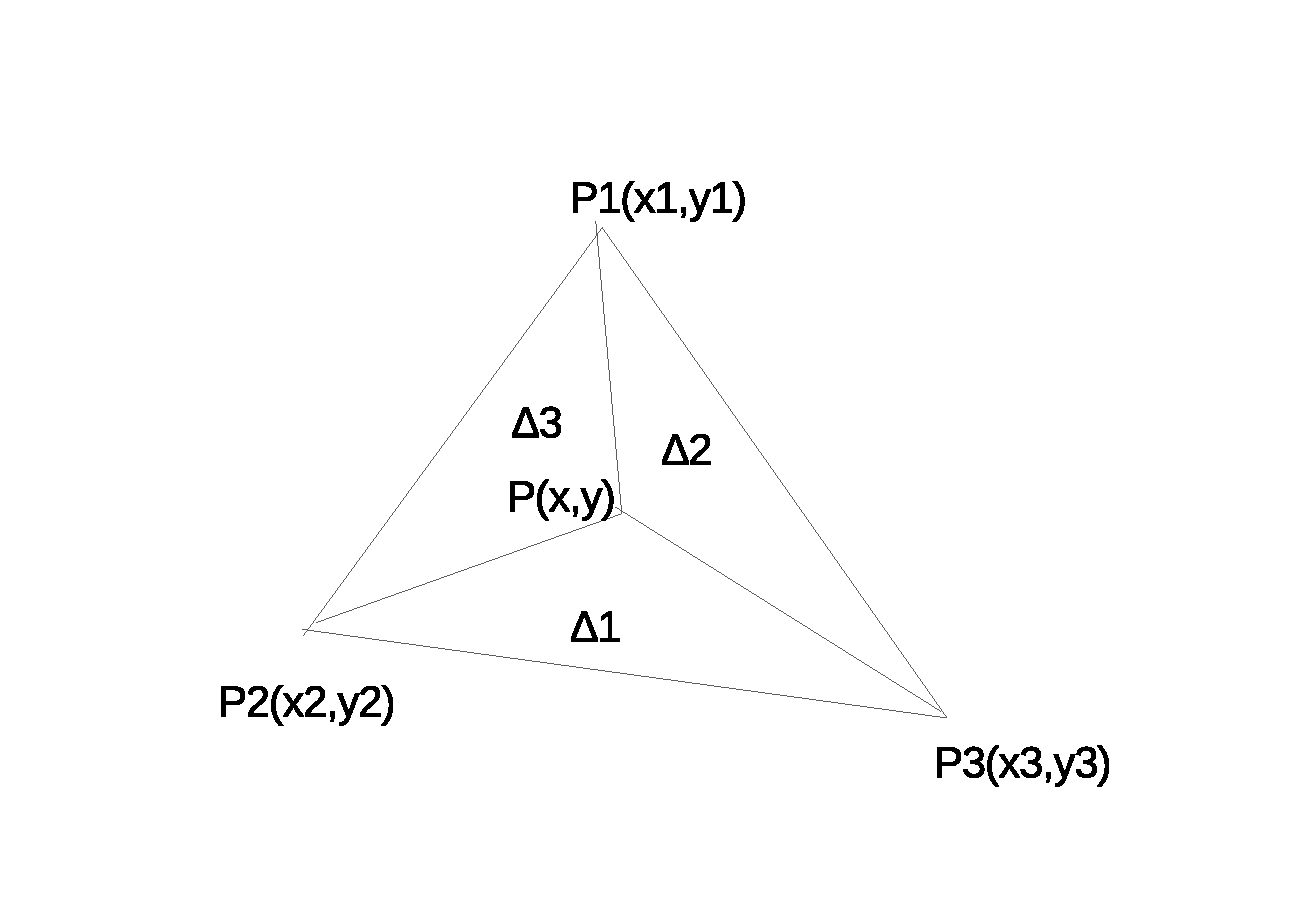
\includegraphics[width=10cm]{area_coordinates.eps}
\caption{三角形要素と三つの小三角形領域}
\end{center}
\end{figure}

図1の三角形要素に注目する。三角形要素内の任意の1点$P(x,y)$と
3頂点$P_1,P_2,P_3$をそれぞれ直線で繋いで要素内を三つの小三角形領域に分割する。

\begin{center}
\begin{tabular}{lll}
  $頂点a$&...&$P_1(x_1,y_1)$\\
  $頂点b$&...&$P_2(x_2,y_2)$\\
  $頂点c$&...&$P_3(x_3,y_3)$\\
  $中点A$&...&$P_4(\frac{x_2+x_3}{2},\frac{y_2+y_3}{2})$\\
  $中点B$&...&$P_5(\frac{x_3+x_1}{2},\frac{y_3+y_1}{2})$\\
  $中点C$&...&$P_6(\frac{x_1+x_2}{2},\frac{y_1+y_2,}{2})$\\
  $\Delta_1$&...&小三角形$PP_2 P_3$の面積\\
  $\Delta_2$&...&小三角形$PP_3 P_1$の面積\\
  $\Delta_3$&...&小三角形$PP_1 P_2$の面積\\
  $\Delta_e$&...&三角形$P_1 P_2 P_3$の面積
\end{tabular}
\end{center}

\begin{equation}
\displaystyle
L_1 = \frac{\Delta_1}{\Delta_e},
L_2 = \frac{\Delta_2}{\Delta_e},
L_3 = \frac{\Delta_3}{\Delta_e}
\end{equation}


定義式(20)のように$L_1, L_2, L_3$を定義すると、この3つのスカラーの間には
次の関係式が成り立つ。

\begin{equation}
\displaystyle
L_1 + L_2 + L_3 = 1
\end{equation}

$(L_1,L_2,L_3)$を面積座標と呼ぶ。



\begin{center}
\begin{tabular}{llll}
  $頂点a$&...&$P_1(x_1,y_1)$&=面積座標(1,0,0)\\
  $頂点b$&...&$P_2(x_2,y_2)$&=面積座標(0,1,0)\\
  $頂点c$&...&$P_3(x_3,y_3)$&=面積座標(0,0,1)\\
  $中点A$&...&$P_4(\frac{x_2+x_3}{2},\frac{y_2+y_3}{2})$&$=面積座標(0,\frac{1}{2},\frac{1}{2})$\\
  $中点B$&...&$P_5(\frac{x_3+x_1}{2},\frac{y_3+y_1}{2})$&$=面積座標(\frac{1}{2},0,\frac{1}{2})$\\
  $中点C$&...&$P_6(\frac{x_1+x_2}{2},\frac{y_1+y_2,}{2})$&$=面積座標(\frac{1}{2},\frac{1}{2},0)$
\end{tabular}
\end{center}


\begin{equation}
  \Delta_e = \frac{1}{2}\left|\begin{array}{ccc}
  1&1&1\\
  x_1&x_2&x_3\\
  y_1&y_2&y_3
  \end{array}\right|=x_1 y_2 + x_2 y_3 + x_3 y_1- y_1 x_2 - y_2 x_3 - y_3 x_1
\end{equation}


\begin{equation}
  \Delta_1 = \frac{1}{2}\left|\begin{array}{ccc}
  1&1&1\\
  x&x_2&x_3\\
  y&y_2&y_3
  \end{array}\right|=x y_2 + x_2 y_3 + x_3 y- y x_2 - y_2 x_3 - y_3 x
\end{equation}


\begin{equation}
  \Delta_2 = \frac{1}{2}\left|\begin{array}{ccc}
  1&1&1\\
  x_1&x&x_3\\
  y_1&y&y_3
  \end{array}\right|=x_1 y + x y_3 + x_3 y_1- y_1 x - y x_3 - y_3 x_1
\end{equation}


\begin{equation}
  \Delta_3 = \frac{1}{2}\left|\begin{array}{ccc}
  1&1&1\\
  x_1&x_2&x\\
  y_1&y_2&y
  \end{array}\right|=x_1 y_2 + x_2 y + x y_1- y_1 x_2 - y_2 x - y x_1
\end{equation}

\begin{equation}
  L_1 = \frac{\Delta_1}{\Delta_e} = \frac{(y_2-y_3)x-(x_2-x_3)y +x_2 y_3 - y_2 x_3}{\Delta_e}
\end{equation}


\begin{equation}
  L_2 = \frac{\Delta_1}{\Delta_e} = \frac{(y_1-y_2)x-(x_1-x_2)y +x_1 y_2 - y_1 x_2}{\Delta_e}
\end{equation}


\begin{equation}
  L_3 = \frac{\Delta_1}{\Delta_e} = \frac{(y_3-y_1)x-(x_3-x_1)y +x_3 y_1 - y_3 x_1}{\Delta_e}
\end{equation}

$L_1, L_2, L_3$を具体的に計算した。
それぞれ$x,y$の一次関数であることが見て取れる。

\section{形状関数ベクトル}



\subsection{1次要素}
\begin{equation}
  K_e = \left\{\begin{array}{c}
      L_1\\
      L_2\\
      L_3
  \end{array}\right\} = \left\{\begin{array}{c}
  \frac{1}{\Delta e}\left\{(y_2-y_3)x-(x_2-x_3)y +x_2 y_3 - y_2 x_3\right\}\\
  \frac{1}{\Delta e}\left\{(y_3-y_1)x-(x_3-x_1)y +x_3 y_1 - y_3 x_1\right\}\\
  \frac{1}{\Delta e}\left\{(y_1-y_2)x-(x_1-x_2)y +x_1 y_2 - y_1 x_2\right\}\\
  \end{array}\right\}
\end{equation}

\subsection{2次要素}
\begin{equation}
N_e = \left\{\begin{array}{c}
      L_1(2L_1-1)\\
      L_2(2L_2-1)\\
      L_3(2L_3-1)\\
      4L_2L_3\\
      4L_3L_1\\
      4L_1L_2
\end{array}\right\}
\end{equation}
\[
  L_1(2L_1-1)= \frac{1}{\Delta_e^2}\left\{
  2(y_2-y_3)^2x^2+2(x_2-x_3)^2y^2-4(x_2-x_3)(y_2-y_3)xy\right.
\]
\[\left.
+(y_2-y_3)(4x_2y_3-4y_2x_3-1)x-(x_2-x_3)(4x_2y_3-4x_2y_3-1)y+(x_2y_3-y_2x_3)(2x_2y_3-2y_2x_3-1)\right\}
\]

\[
  L_2(2L_2-1)= \frac{1}{\Delta_e^2}\left\{
  2(y_3-y_1)^2x^2+2(x_3-x_1)^2y^2-4(x_3-x_1)(y_3-y_1)xy\right.
\]
\[\left.
+(y_3-y_1)(4x_3y_1-4y_3x_1-1)x-(x_3-x_1)(4x_3y_1-4x_3y_1-1)y+(x_3y_1-y_3x_1)(2x_3y_1-2y_3x_1-1)\right\}
\]

\[
  L_3(2L_3-1)= \frac{1}{\Delta_e^2}\left\{
  2(y_1-y_2)^2x^2+2(x_1-x_2)^2y^2-4(x_1-x_2)(y_1-y_2)xy\right.
\]
\[\left.
+(y_1-y_2)(4x_1y_2-4y_1x_2-1)x-(x_1-x_2)(4x_1y_2-4x_1y_2-1)y+(x_1y_2-y_1x_2)(2x_1y_2-2y_1x_2-1)\right\}
\]


\[
4L_2L_3 = \frac{4}{\Delta_e^2}\left\{ (y_3-y_1)(y_1-y_2)x^2+(x_3-x_1)(x_1-x_2)y^2
\right.\]\[\left.
-((y_3-y_1)(x_1-x_2)+(x_3-x_1)(y_1-y_2))xy
+((y_3-y_1)(x_1x_2-y_1y_2)+(y_1-y_2)(x_3y_1-y_3x_1))x
\right.\]\[\left.
-((x_3-x_1)(x_1y_2-y1x_2)+(x_1-y_2)(x_3y_1-y_3x_1))y+(x_3y_1-y_3x_1)(x_1y_2-y1_x2) \right\}
\]


\[
4L_3L_1 = \frac{4}{\Delta_e^2}\left\{ (y_1-y_2)(y_2-y_3)x^2+(x_1-x_2)(x_2-x_3)y^2
\right.\]\[\left.
-((y_1-y_2)(x_2-x_3)+(x_1-x_2)(y_2-y_3))xy
+((y_1-y_2)(x_2x_3-y_2y_3)+(y_2-y_3)(x_1y_2-y_1x_2))x
\right.\]\[\left.
-((x_1-x_2)(x_2y_3-y_2x_3)+(x_2-y_3)(x_1y_2-y_1x_2))y+(x_1y_2-y_1x_2)(x_2y_3-y2_x3) \right\}
\]


\[
4L_1L_2 = \frac{4}{\Delta_e^2}\left\{ (y_2-y_3)(y_3-y_1)x^2+(x_2-x_3)(x_3-x_1)y^2
\right.\]\[\left.
-((y_2-y_3)(x_3-x_1)+(x_2-x_3)(y_3-y_1))xy
+((y_2-y_3)(x_3x_1-y_3y_1)+(y_3-y_1)(x_2y_3-y_2x_3))x
\right.\]\[\left.
-((x_2-x_3)(x_3y_1-y_3x_1)+(x_3-y_1)(x_2y_3-y_2x_3))y+(x_2y_3-y_2x_3)(x_3y_1-y3_x1) \right\}
\]


1次要素は$x,y$の1次関数、2次要素は$x,y$の2次関数になっている。
また、$\Delta_e$は領域$\Omega_e$の面積である。

\section{C++プログラムとの対応}

\begin{verbatim}
  typedef struct{ double x, y; char *label; } xyc;
  typedef struct{ int a, b, c, A, B, C; } nde;
\end{verbatim}

xyc(xy coordinate)が節点-座標対応表、nde(node)が要素-節点対応表である。
ここに要素-節点対応表Nの要素eに対して、以下の表記がプログラムで成される。
また、Zは節点-座標対応表の(Zahyou)である

節点-座標対応表における *labelには、境界条件を表す文字列が入っており、
これを参照することによって、境界条件を実現することが出来る。

\begin{center}
\begin{tabular}{lllllll}
  $頂点a$&...&N[e].a&P(Z[N[e].a].x,Z[N[e].a].y)&$P_1(x_1,y_1)$&=面積座標(1,0,0)\\
  $頂点b$&...&N[e].b&P(Z[N[e].b].x,Z[N[e].b].y)&$P_2(x_2,y_2)$&=面積座標(0,1,0)\\
  $頂点c$&...&N[e].c&P(Z[N[e].c].x,Z[N[e].c].y)&$P_3(x_3,y_3)$&=面積座標(0,0,1)\\
  $中点A$&...&N[e].A&P(Z[N[e].A].x,Z[N[e].A].y)&$P_4(\frac{x_2+x_3}{2},\frac{y_2+y_3}{2})$&$=面積座標(0,\frac{1}{2},\frac{1}{2})$\\
  $中点B$&...&N[e].B&P(Z[N[e].B].x,Z[N[e].B].y)&$P_5(\frac{x_3+x_1}{2},\frac{y_3+y_1}{2})$&$=面積座標(\frac{1}{2},0,\frac{1}{2})$\\
  $中点C$&...&N[e].C&P(Z[N[e].C].x,Z[N[e].C].y)&$P_6(\frac{x_1+x_2}{2},\frac{y_1+y_2,}{2})$&$=面積座標(\frac{1}{2},\frac{1}{2},0)$
\end{tabular}
\end{center}


例えば、以下のようにC++関数 dalta()を定義し、適切に設定されているZ,Nを用いると、
De = delta(e,Z,N);とすることによって、要素eの面積を変数Deにセットすることが出来る。


\begin{verbatim}
double delta(int i, vector<xyc>&Z, vector<nde>&N)
{
  double xi, xj, xk, yi, yj, yk;

  xi = Z[N[i].a].x;
  xj = Z[N[i].b].x;
  xk = Z[N[i].c].x;
  yi = Z[N[i].a].y;
  yj = Z[N[i].b].y;
  yk = Z[N[i].c].y;
  return (xi*yj+xj*yk+xk*yi-yi*xj-yj*xk-yk*xi)/2.0;
}
\end{verbatim}


有限要素メッシュZ,Nを矛盾なく構成することは、一般に労力がかかる。要素数数百程度のものであっても、
方眼紙に製図していき、座標を拾っていく作業は、慣れもあるだろうが、突貫工事でやったとしても1週間はかか
るであろう。
この単純ではあるが、ミスの許されない作業をプログラムで自動化しようというのは自然な欲求である。

URL\footnote{https://github.com/naruto2/femesh.git}
の注には、デローニー法を用いた要素自動分割のプログラムが利用出来る形で用意されている。


\section{弱形式の離散化の続き}

速度成分$u,v$に対する形状関数ベクトルを${\bf N}_e$、
圧力$p$に対する形状関数ベクトルを${\bf K}_e$とし、
三角形領域内部$\Omega_e$で、以下のように置き換える。

\begin{equation}
u = {\bf N}_e^T{\bf U}_e, ~~~ v = {\bf N}_e^T{\bf V}_e, ~~~ p = {\bf K}_e^T{\bf P}_e
\end{equation}


ここに、${\bf U}_e,{\bf V}_e,{\bf P}_e$はそれぞれ$u,v,p$の節点における値を成分とするベクトルである。
また、重み関数についても同様に以下のように表す。

\begin{equation}
u^* = {\bf N}_e^T{\bf U}_e^*, ~~~ v^* = {\bf N}_e^T{\bf V}_e^*, ~~~ p^* = {\bf K}_e^T{\bf P}_e^*
\end{equation}



式(31)、(32)をナビエ・ストークス方程式の弱形式(17)(18)と連続の方程式の弱形式(19)に代入すると
次のようになる。

\[
\sum_{e=1}^N\left[ \int\int_{\Omega_e}{\bf N}_e^T{\bf U}_e^*(\frac{\partial{\bf N}_e^T}{\partial t}
  + {\bf N}_e^T{\bf U}_e\frac{\partial {\bf N}_e^T{\bf U}_e}{\partial x}
  + {\bf N}_e^T{\bf V}_e\frac{\partial {\bf N}_e^T{\bf U}_e}{\partial x})dxdy
\right.\]\[
- \int\int_{\Omega_e}\frac{\partial {\bf N}_e^T{\bf U}_e^*}{\partial x}{\bf K}_e^T {\bf P}_e dxdy
\]\[
+\frac{1}{Re}\int\int_{\Omega_e}(
\frac{\partial {\bf N}_e^T{\bf U}_e^*}{\partial x}\frac{\partial {\bf N}_e^T{\bf U}_e}{\partial x}
\frac{\partial {\bf N}_e^T{\bf U}_e^*}{\partial y}\frac{\partial {\bf N}_e^T{\bf U}_e}{\partial y}
)dxdy
\]\begin{equation}
\left.-\int\int_{\Omega_e}{\bf N}_e^T{\bf U}_e^* X dxdy \right] = 0
\end{equation}

\[
\sum_{e=1}^N\left[ \int\int_{\Omega_e}{\bf N}_e^T{\bf V}_e^*(\frac{\partial{\bf N}_e^T}{\partial t}
  + {\bf N}_e^T{\bf U}_e\frac{\partial {\bf N}_e^T{\bf V}_e}{\partial x}
  + {\bf N}_e^T{\bf V}_e\frac{\partial {\bf N}_e^T{\bf V}_e}{\partial x})dxdy
\right.\]\[
- \int\int_{\Omega_e}\frac{\partial {\bf N}_e^T{\bf V}_e^*}{\partial x}{\bf K}_e^T {\bf P}_e dxdy
\]\[
+\frac{1}{Re}\int\int_{\Omega_e}(
\frac{\partial {\bf N}_e^T{\bf V}_e^*}{\partial x}\frac{\partial {\bf N}_e^T{\bf V}_e}{\partial x}
\frac{\partial {\bf N}_e^T{\bf V}_e^*}{\partial y}\frac{\partial {\bf N}_e^T{\bf V}_e}{\partial y}
)dxdy
\]\begin{equation}
\left.-\int\int_{\Omega_e}{\bf N}_e^T{\bf V}_e^* X dxdy \right] = 0
\end{equation}


\begin{equation}
  \sum_{e=1}^N\left[ \int\int_{\Omega_e}{\bf K}_e^T{\bf P}_e^*(
    \frac{\partial {\bf N}_e^T{\bf U}_e}{\partial x}
    \frac{\partial {\bf N}_e^T{\bf V}_e}{\partial y}
    )dxdy\right]=0
\end{equation}


ここで、${\bf M}_e, {\bf A}_e({\bf U}_e,{\bf V}_e), {\bf D}_e, {\bf H}_{xe}, {\bf H}_{ye}, {\bf F}_{xe}, {\bf F}_{ye}$を以下のように定義する。

\begin{eqnarray}
  {\bf M}_e&=&\int\int_{\Omega_e}{\bf N}_e{\bf N}_e^Tdxdy \\
  {\bf A}_e({\bf U}_e,{\bf V}_e) &=& \int\int_{\Omega_e}{\bf N}_e(
  {\bf N}_e^T{\bf U}_e\frac{\partial {\bf N}_e^T}{\partial x}
 + {\bf N}_e^T{\bf V}_e\frac{\partial {\bf N}_e^T}{\partial y}
  )dxdy\\
 {\bf D}_e&=&\int\int_{\Omega_e}(
 \frac{\partial{\bf N}_e}{\partial x}\frac{\partial{\bf N}_e^T}{\partial x}
+\frac{\partial{\bf N}_e}{\partial y}\frac{\partial{\bf N}_e^T}{\partial y}
 )dxdy\\
{\bf H}_{xe}&=&\int\int_{\Omega_e}\frac{\partial {\bf N}_e}{\partial x}{\bf K}_e^Tdxdy\\
{\bf H}_{ye}&=&\int\int_{\Omega_e}\frac{\partial {\bf N}_e}{\partial y}{\bf K}_e^Tdxdy\\
{\bf F}_{xe}&=&\int\int_{\Omega_e}{\bf N}_eXdxdy\\
{\bf F}_{ye}&=&\int\int_{\Omega_e}{\bf N}_eYdxdy
\end{eqnarray}

(34)(35)(36)にこれらを代入して整理する。${\bf N}_e^T{\bf U}_e^* = ({\bf U}_e^*)^T{\bf N}_e$及び
$\frac{\partial}{\partial t} = \frac{d}{dt}$も用いる。


\begin{eqnarray}
  \sum_{e=1}^N({\bf U}_e^*)^T\left[{\bf M}_e\frac{d{\bf U}_e}{dt}+{\bf A}_e({\bf U}_e,{\bf V}_e){\bf U}_e
-{\bf H}_{xe}{\bf P}_e+\frac{1}{Re}{\bf D}_e{\bf U}_e-{\bf F}_{xe}\right]=0\\
  \sum_{e=1}^N({\bf V}_e^*)^T\left[{\bf M}_e\frac{d{\bf V}_e}{dt}+{\bf A}_e({\bf U}_e,{\bf V}_e){\bf V}_e
-{\bf H}_{ye}{\bf P}_e+\frac{1}{Re}{\bf D}_e{\bf U}_e-{\bf F}_{ye}\right]=0\\
  \sum_{e=1}^N({\bf P}_e^*)^T\left[{\bf H}_{xe}^T{\bf U}_e+{\bf H}_{ye}^T{\bf V}_e\right]=0
\end{eqnarray}

重みベクトル${\bf U}_e^*,{\bf V}_e^*,{\bf P}_e^*$の任意性を考慮して、(43)(44)(45)式の
大括弧内がゼロベクトルに等しいと置くと、$1\leq e\leq N$なる要素eに対して、
以下の式が成り立つ。


\begin{eqnarray}
 {\bf M}_e\frac{d{\bf U}_e}{dt}+{\bf A}_e({\bf U}_e,{\bf V}_e){\bf U}_e
-{\bf H}_{xe}{\bf P}_e+\frac{1}{Re}{\bf D}_e{\bf U}_e-{\bf F}_{xe}={\bf 0}\\
 {\bf M}_e\frac{d{\bf V}_e}{dt}+{\bf A}_e({\bf U}_e,{\bf V}_e){\bf V}_e
-{\bf H}_{ye}{\bf P}_e+\frac{1}{Re}{\bf D}_e{\bf U}_e-{\bf F}_{ye}={\bf 0}\\
 {\bf H}_{xe}^T{\bf U}_e+{\bf H}_{ye}^T{\bf V}_e={\bf 0}
\end{eqnarray}

ここで、要素-節点対応表から要素1について具体的に計算してみる。
\begin{verbatim}
cavity32.mesh ... 要素数2052 頂点節点数1091
<nde>
   1    34    1    2  1092 1093 1094
   2     2    3   36  1095 1096 1097
   3     3    4   37  1098 1099 1100
   4     4    5   38  1101 1102 1103
   5     5    6   39  1104 1105 1106
   (続く)
\end{verbatim}
上記の表より、要素1を構成する節点番号は $(a,b,c,A,B,C)=(34,1,2,1092,1093,1094)$であることがわかる。
${\bf M}$を(頂点節点数+中点節点数)元の正方行列とすると、

\[
\left[\begin{array}{cccccc}
m_{[34][34]} & m_{[34][1]} & m_{[34][2]} & m_{[34][1092]} & m_{[34][1093]} & m_{[34][1094]}\\
m_{[ 1][34]} & m_{[1][1]} & m_{[1][2]} & m_{[1][1092]} & m_{[1][1093]} & m_{[1][1094]}\\
m_{[ 2][34]} & m_{[2][1]} & m_{[2][2]} & m_{[2][1092]} & m_{[2][1093]} & m_{[2][1094]}\\
m_{[1092][34]} & m_{[1092][1]} & m_{[1092][2]} & m_{[1092][1093]} & m_{[1092][1093]}&m_{[1092][1094]}\\
m_{[1093][34]} & m_{[1093][1]} & m_{[1093][2]} & m_{[1093][1093]} & m_{[1093][1093]}&m_{[1093][1094]}\\
m_{[1094][34]} & m_{[1094][1]} & m_{[1094][2]} & m_{[1094][1093]} & m_{[1094][1093]}&m_{[1094][1094]}
\end{array}\right]
\]

\[
=\int\int_{\Omega_1}{\bf N}_1{\bf N}_1^Tdxdy 
\]


\[
=\int\int_{\Omega_1}\left\{\begin{array}{c}
L_{34}(2L_{34}-1)\\
L_{1}(2L-{1}-1)\\
L_{2}(2L_{2}-1)\\
4L_{1}L_{2}\\
4L_{34}L_{1}\\
4L_{2}L_{34}
\end{array}\right\}(
L_{34}(2L_{34}-1),
L_{1}(2L-{1}-1),
L_{2}(2L_{2}-1),
4L_{1}L_{2},
4L_{34}L_{1},
4L_{2}L_{34}
)dxdy 
\]


\[
=\int\int_{\Omega_1}\left\{\begin{array}{c}
a\\
b\\
c\\
A\\
B\\
C
\end{array}\right\}(
a,b,c,A,B,C
)dxdy 
\]

\[
=\int\int_{\Omega_1}\left[\begin{array}{cccccc}
    a^2&ab&ac&aA&aB&aC\\
    ba&b^2&bc&bA&bB&bC\\
    ca&cb&c^2&cA&cB&cC\\
    Aa&Ab&Ac&A^2&AB&AC\\
    Ba&Bb&Bc&BA&B^2&BC\\
    Ca&Cb&Cc&CA&CB&C^2
\end{array}\right]dxdy
\]



\[
=\left[\begin{array}{cccccc}
    \int\int_{\Omega_1}a^2dxdy&\int\int_{\Omega_1}abdxdy&\int\int_{\Omega_1}acdxdy&\int\int_{\Omega_1}aAdxdy&\int\int_{\Omega_1}aBdxdy&\int\int_{\Omega_1}aCdxdy\\
    \int\int_{\Omega_1}badxdy&\int\int_{\Omega_1}b^2dxdy&\int\int_{\Omega_1}bcdxdy&\int\int_{\Omega_1}bAdxdy&\int\int_{\Omega_1}bBdxdy&\int\int_{\Omega_1}bCddxdy\\
    \int\int_{\Omega_1}cadxdy&\int\int_{\Omega_1}cbdxdy&\int\int_{\Omega_1}c^2dxdy&\int\int_{\Omega_1}cAdxdy&\int\int_{\Omega_1}cBdxdy&\int\int_{\Omega_1}cCdxdy\\
    \int\int_{\Omega_1}Aadxdy&\int\int_{\Omega_1}Abdxdy&\int\int_{\Omega_1}Acdxdy&\int\int_{\Omega_1}A^2dxdy&\int\int_{\Omega_1}ABdxdy&\int\int_{\Omega_1}ACddxdy\\
    \int\int_{\Omega_1}Badxdy&\int\int_{\Omega_1}Bbdxdy&\int\int_{\Omega_1}Bcdxdy&\int\int_{\Omega_1}BAdxdy&\int\int_{\Omega_1}B^2dxdy&\int\int_{\Omega_1}BCdxdy\\
    \int\int_{\Omega_1}Cadxdy&\int\int_{\Omega_1}Cbdxdy&\int\int_{\Omega_1}Ccdxdy&\int\int_{\Omega_1}CAdxdy&\int\int_{\Omega_1}CBdxdy&\int\int_{\Omega_1}C^2ddxdy
\end{array}\right]
\]


\end{document}
